\documentclass{standalone}
\usepackage[T1]{fontenc}
\usepackage[latin2]{inputenc}
\usepackage[english]{babel}
\usepackage{tikz}
\usepackage{times}
\usetikzlibrary{calc,through,backgrounds,positioning,fit,mindmap}
\usetikzlibrary{shapes,arrows,shadows}
 
\begin{document}
 


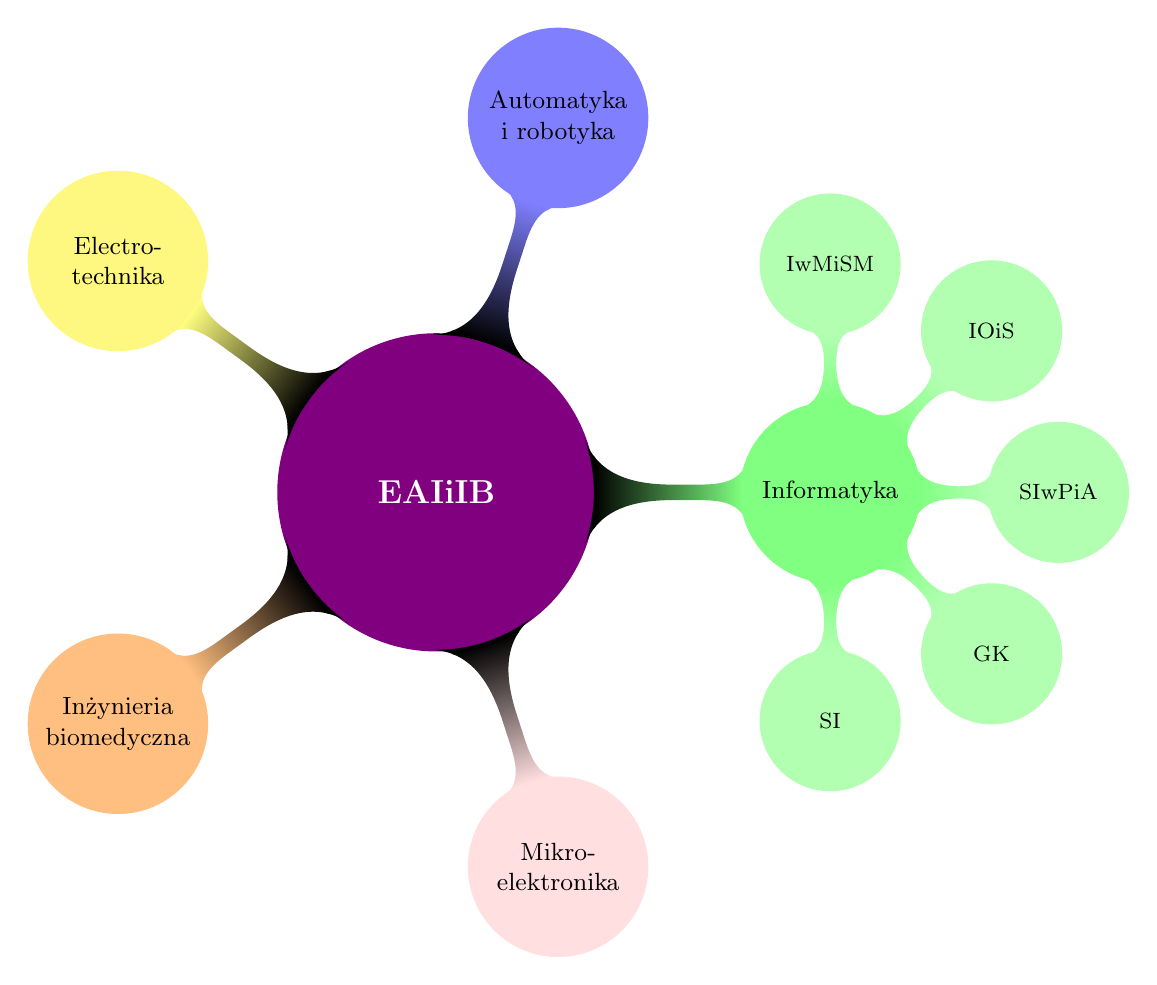
\begin{tikzpicture}[mindmap]

\node [concept,concept color=red!50!blue, text=white] {\bf EAIiIB}
  child[grow=0, concept color=green!50] {node[concept] {Informatyka}
    child[grow=90, concept color=green!30] {node[concept] {IwMiSM}}
    child[grow=45, concept color=green!30] {node[concept] {IOiS}}  
    child[grow=0, concept color=green!30] {node[concept] {SIwPiA}}  
    child[grow=315, concept color=green!30] {node[concept] {GK}}  
    child[grow=270, concept color=green!30] {node[concept] {SI}}  
  }
  child[grow=72, concept color=blue!50] {node[concept] {Automatyka i robotyka}}
  child[grow=144, concept color=yellow!50] {node[concept] {Electro-technika}}
  child[grow=216, concept color=orange!50] {node[concept] {In{\.z}ynieria biomedyczna}}
  child[grow=288, concept color=pink!50] {node[concept] {Mikro-elektronika}}
;

\end{tikzpicture}

 
\end{document}
